\chapter{\label{ch:ch4} Design ad Implementation}

This chapter outlines the design and implementation phases of the mobile robot system project. The purpose of this chapter is to describe the system’s architecture, the design of each subsystem, the integration of hardware and software, and how these components work together to achieve the goals of this project. The design emphasizes ease of navigation, real-time feedback, and effective control via an intuitive interface.

\section{\label{sec:ch4_firstsec}System Design}

The design of the mobile robot system was based on the specific project requirements outlined in Chapter\ref{ch:req_and_specs}. Following a detailed review of relevant literature and an analysis of system needs, the robot’s overall design was established. The architecture integrates several key components—Raspberry Pi, camera module, fiducial markers, motor control system, and wireless communication modules—to ensure optimal system performance.

The core decision-making process involved selecting the appropriate technologies and components. Based on the findings from previous research (e.g., Jacobsen et al. \cite{jacobsen2018}, La Delfa et al. \cite{delfa2015}, and Vanitha et al. \cite{vanitha2016}), which explored various mobile robot control methods using augmented reality (AR) and computer vision, it became clear that a Raspberry Pi-based system with a web interface would provide the required flexibility and ease of control for this project.

After evaluating several options for actuation and navigation, it was determined that motorized control through a motor driver and a four-wheel drive system would provide the most reliable and efficient solution for movement. This decision was supported by studies that demonstrate the performance of motor-driven robots in both laboratory and dynamic environments. Additionally, the use of fiducial markers, such as ArUco or AprilTag markers, was identified as a robust solution for localization and obstacle avoidance (La Delfa et al. \cite{delfa2015}; Vanitha et al. \cite{vanitha2016}).

The integration of these components into a cohesive design was a critical aspect of the project. The Raspberry Pi was chosen as the central processing unit because of its ability to handle computer vision tasks and interface with the hardware seamlessly. The camera module was selected to provide real-time video streaming, which not only serves as an input for the robot’s environment perception but also allows for remote monitoring through the web interface.

\begin{figure}[H]
	\centering
	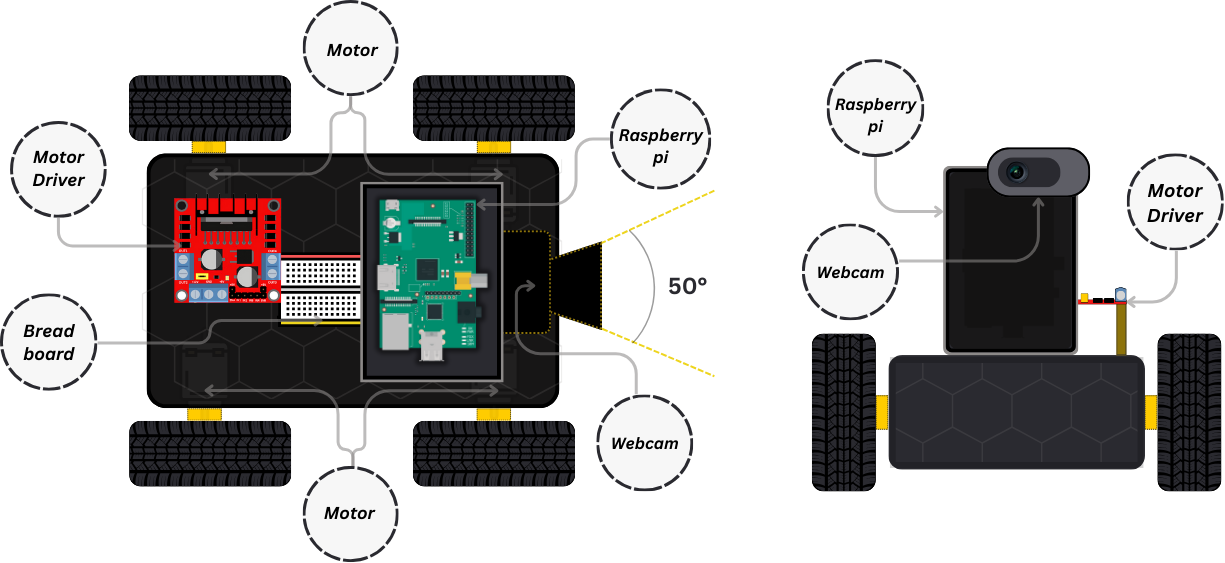
\includegraphics[width=1\textwidth]{ch4/figs/robot_car.png}
	\caption{Illustration of the hardware layout, showing the arrangement of key components like the Raspberry Pi, motor system, and camera module.}
	\label{fig:hardware_layout}
\end{figure}


\section{\label{sec:hardware} Hardware System Architecture}

The system architecture provides a high-level overview of how the robot and its subsystems interact with one another to achieve semi-autonomous navigation, real-time feedback, and remote control functionality. The key components of the system include the hardware modules such as the Raspberry Pi, motors, sensors, and camera, alongside software elements such as computer vision algorithms and the web-based control interface.

The project is composed of several key components, below is a high level overview of all the components that are needed in order execute the project properly.

\section{Microcontroller Selection}

The Raspberry Pi Model 4B with 4GB RAM was selected as the microcontroller for this project due to its versatility and capability to handle multiple complex tasks simultaneously. Its ability to run sophisticated computer vision algorithms while interfacing with other hardware components makes it ideal for this application. The capacity to manage real-time video streaming, marker detection, and motor control simultaneously is crucial for the system's functionality.

Unlike dedicated micro-controllers such as Arduino, the Raspberry Pi can run Python-based frameworks like OpenCV, which is essential for implementing the system's computer vision capabilities. This aligns with findings from Jacobsen et al. \cite{jacobsen2018}, who demonstrated the effectiveness of using a Raspberry Pi for web hosting.

The use of a single, integrated system for both processing and control, as highlighted in Chapter\ref{ch:lit_review}, simplifies the overall design, reduces latency, and enhances system performance. In our setup, the Raspberry Pi functions as the central processing unit, responsible for interfacing with all other components. It processes the video feed from the camera, executes computer vision algorithms such as ArUco marker detection, and transmits control signals to the motor driver. The Raspberry Pi runs a Python-based framework that integrates OpenCV for vision tasks and SocketIO for communication with the web interface. This allows it to receive input from the camera, process it using OpenCV, and then send commands to the motor driver based on the detected environment and user instructions received through the control interface.

The selection of the 4GB RAM version was made to ensure sufficient memory for running multiple processes concurrently and handling intensive computational tasks. While the 8GB version offers more memory, the 4GB model provides a balanced compromise between performance and cost-effectiveness for our application. Table \ref{table:pi_specs} provides a comparison of the specifications for the Raspberry Pi Model 4B with 4GB RAM:


\begin{table}[h!]
	\centering
	\begin{tabular}{|l|c|c|c|}
		\hline
		\textbf{Specification} & \textbf{2GB RAM} & \textbf{4GB RAM} & \textbf{8GB RAM} \\
		\hline
		\textbf{CPU} & Quad-core Cortex-A72 & Quad-core Cortex-A72 & Quad-core Cortex-A72 \\
		\hline
		\textbf{Clock Speed} & 1.5 GHz & 1.5 GHz & 1.5 GHz \\
		\hline
		\textbf{RAM} & 2GB LPDDR4 & 4GB LPDDR4 & 8GB LPDDR4 \\
		\hline
		\textbf{Networking} & Gigabit Ethernet & Gigabit Ethernet & Gigabit Ethernet \\
		\hline
		\textbf{USB Ports} & 2x USB 3.0, 2x USB 2.0 & 2x USB 3.0, 2x USB 2.0 & 2x USB 3.0, 2x USB 2.0 \\
		\hline
		\textbf{Video Output} & 2x micro-HDMI & 2x micro-HDMI & 2x micro-HDMI \\
		\hline
		\textbf{Power Supply} & 5V/3A USB-C & 5V/3A USB-C & 5V/3A USB-C \\
		\hline
	\end{tabular}
	\caption{Comparison of Raspberry Pi Model 4B RAM Versions}
	\label{table:pi_specs}
\end{table}

This hardware configuration provides the necessary processing power and memory to handle the computer vision tasks, video streaming, and robot control required by our project. The Raspberry Pi 4B with 4GB RAM offers a robust platform capable of running complex algorithms, processing real-time video data, and managing the various input and output operations essential for the robot car's operation.

\subsection{Camera Module}
The camera plays a pivotal role in this system as it provides real-time feedback necessary for detecting fiducial markers and controlling the robot's movement. The decision to use a high-resolution web camera, specifically the HD Logitech C270, over a more basic sensor was based on the need for precise marker detection, which demands high-quality image capture. La Delfa et al. \cite{delfa2015} emphasized the importance of high-resolution cameras for accurate marker detection, particularly in dynamic environments. A higher-quality video feed improves the reliability of computer vision algorithms and ensures better control over the robot’s movements.

The camera module continuously captures the video feed, which is streamed to both the user via the web interface and the Raspberry Pi for processing. The camera plays a critical role in detecting fiducial markers in the environment, enabling navigation and interaction based on visual feedback.

\begin{table}[h!]
	\centering
	\caption{Comparison between Logitech C270 and Raspberry Pi Camera Module}
	\begin{tabular}{|p{4cm}|>{\centering\arraybackslash}p{5cm}|>{\centering\arraybackslash}p{5cm}|}
		\hline
		\textbf{Specification} & \textbf{Logitech C270}               & \textbf{Raspberry Pi Camera Module V2} \\ \hline
		Resolution             & 1280x720 (HD)                        & 3280x2464 (8 MP)                       \\ \hline
		Frame Rate             & 30 fps (at 720p)                     & 30 fps (at 1080p)                      \\ \hline
		Field of View (FOV)    & 60°                                  & 62.2°                                  \\ \hline
		Interface              & USB                                  & CSI (Camera Serial Interface)          \\ \hline
		Price                  & readily-available                             & Low                                    \\ \hline
		Ease of Use            & Plug-and-play                        & Requires configuration                 \\ \hline
		Compatibility          & Universal (works on various systems) & Raspberry Pi exclusive                 \\ \hline
	\end{tabular}
	\label{tab:camera_comparison}
\end{table}


The Logitech C270 was chosen primarily due to it being readily available for use and its ability to seamlessly integrate into various systems via USB, requiring minimal configuration compared to the Raspberry Pi Camera Module. Additionally, while the Raspberry Pi camera offers higher resolution, the Logitech C270 provides sufficient image quality for marker detection. Furthermore, the webcam is universally compatible, making it a practical choice for prototyping and development in this context.

The camera module continuously captures the video feed, which is streamed to both the user via the web interface and the Raspberry Pi for processing. The camera plays a critical role in detecting fiducial markers in the environment, enabling navigation and interaction based on visual feedback.

\subsection{Motor and Drive System}

The four-wheel drive system of the DGU ALUM MULTI-CHASSIS 4WD KIT was selected to ensure that the robot can move with precision across various terrains. This chassis provides a sturdy foundation for the robot's movement capabilities. The motors used in this system operate on 3V\textasciitilde12VDC, with a maximum torque of 800gf cm MIN at 3V and a no-load speed of 1:48 at 3V. Each motor measures 7x2.2x1.8cm and draws a load current of 70mA (250mA MAX) at 3V. The use of an L298N H-bridge motor driver allows for efficient control of these motors via Pulse Width Modulation (PWM) signals from the Raspberry Pi, enabling fine-grained control over the speed and direction of each motor.

According to Vanitha et al. \cite{vanitha2016}, a robust motor and drive system is essential for mobile robots that rely on real-time feedback from sensors for navigation. The choice of using an H-bridge for motor control is well-supported in robotics literature as it allows for both forward and reverse motion, as well as braking, without adding unnecessary complexity. The four-wheel drive system enables the robot's movement and maneuvering, with the L298N motor driver controlling the speed and direction of the motors based on the PWM signals received from the Raspberry Pi. This setup allows the system to adjust motor power dynamically to maintain proper navigation based on sensor input or user commands, achieving precise movement in various scenarios.

\begin{figure}[H]
	\centering

		\centering
		\includegraphics[width=0.835\textwidth]{ch4/figs/H-Bridge-Interface.png}
		\caption{Illustration of the H-Bridge connection with the motors.}
		\label{fig:motor_H-bridge_connection}
	\end{figure}


\begin{table}[h]
	\centering
	\begin{tabular}{|c|c|c|c|c|c|c|}
		\hline
		\textbf{IN1} & \textbf{IN2} & \textbf{IN3} & \textbf{IN4} & \textbf{Motor A/B} & \textbf{Motor C/D} & \textbf{Robot Movement} \\
		\hline
		0 & 1 & 0 & 1 & Forward & Forward & Forward \\
		\hline
		1 & 0 & 1 & 0 & Reverse & Reverse & Reverse \\
		\hline
		0 & 1 & 1 & 0 & Forward & Reverse & Right Turn \\
		\hline
		1 & 0 & 0 & 1 & Reverse & Forward & Left Turn \\
		\hline
		0 & 0 & 0 & 0 & Stop & Stop & Stop \\
		\hline
		1 & 1 & 1 & 1 & Brake & Brake & Brake \\
		\hline
	\end{tabular}
	\caption{Truth Table for L298N H-Bridge Motor Control}
	\label{tab:condensed_hbridge_control}
\end{table}

The Raspberry Pi generates PWM (Pulse Width Modulation) signals through its GPIO pins, which are connected to the input pins (IN1, IN2, IN3, IN4) of the L298N H-bridge motor driver. These digital signals control the direction and speed of the motors. The H-bridge then interprets these signals and converts them into the appropriate voltage levels and current flow to drive the motors. For Motors A and B, IN1 and IN2 control their direction and speed, while IN3 and IN4 control Motors C and D. The H-bridge acts as an intermediary, amplifying the low-power signals from the Raspberry Pi into the higher power (by using an external power source) needed to drive the DC motors effectively. This setup allows for precise control over each motor's behavior, enabling complex movements of the robot through simple digital commands from the Raspberry Pi.

\section{Power Supply}

Although the primary focus of this project is the robot's navigation, control systems, and augmented reality (AR) integration, the power supply plays a vital role in ensuring reliable performance for the entire system. Without a stable and appropriate power source, the Raspberry Pi, motors, and other components would fail to operate consistently, which could result in unpredictable robot behavior. To address the varying power needs of the system components, two separate power supplies were implemented.

\subsection{Raspberry Pi Power Supply}
The Raspberry Pi requires a consistent and stable power supply to handle its computational tasks, including image processing, web-based control, and communication with other subsystems. A power bank was selected for this purpose due to its wide availability, ease of use, and sufficient power output.

\begin{itemize}
	\item \textbf{Power Source:} A commercial power bank with a 2.1A output was utilized to meet the power requirements of the Raspberry Pi 4.
	
	\item \textbf{Reason for Choice:} The Raspberry Pi 4 requires a power supply that can provide at least \textbf{5V and 3A} for optimal performance. While the chosen power bank offers slightly lower current (2.1A), testing showed that it was sufficient for running the robot's tasks without significant performance degradation. Additionally, the portability and long-lasting capacity of the power bank make it ideal for mobile robotics applications.
	
	\item \textbf{Justification:} Based on several studies on mobile robot systems, power banks are commonly employed due to their flexibility and ability to deliver steady voltage, especially in outdoor or mobile environments. This setup also avoids the need for complex, custom-made power circuits that would otherwise add unnecessary complexity to the system.
\end{itemize}

\subsection{H-Bridge and Motor Power Supply}
The L298N H-bridge motor driver and the motors require a different power supply than the Raspberry Pi, given their higher power demands during operation, particularly under load (e.g., when turning or climbing). To meet this requirement, an RS PRO 3C 3S1P Li-Ion Battery Pack was chosen, which offers higher voltage and capacity.

\begin{itemize}
	\item \textbf{Power Source:} The battery pack consists of \textbf{three 18650 Li-Ion cells} connected in series (3S1P configuration), providing a total voltage of \textbf{11.1V} and a capacity of \textbf{2600mAh}.
	
	\item \textbf{Specifications:}
	\begin{itemize}
		\item Voltage: 11.1V
		\item Capacity: 2600mAh
		\item Configuration: 3 x 18650 cells in series
	\end{itemize}
	
	\item \textbf{Reason for Choice:} The L298N H-bridge can handle up to 46V, so 11.1V is well within its operational range. The motors benefit from higher voltage when performing tasks that require more torque, such as sharp turns or accelerating from a stationary position. The 2600mAh capacity ensures that the robot can operate for extended periods before needing a recharge.
	
	\item \textbf{Justification:} As highlighted in the literature, motor-driven robots require a power supply that can deliver sufficient current and voltage, especially when navigating uneven terrain or performing high-torque tasks like turning. The chosen battery pack is a reliable option for robotics applications because it balances compactness, durability, and energy density.
\end{itemize}

\section{\label{sec:software} Software System Architecture}

The bulk of the project relied on software to function, as it serves as the brain of the entire system, orchestrating the communication between hardware components and enabling real-time decision-making. This architecture integrates several critical subsystems including computer vision, motor control, data processing, and network communication. The primary software components were developed in Python due to its versatility and rich library ecosystem, particularly in robotics, image processing (OpenCV), and web development (Flask).


\begin{figure}[H]
	\centering
	
	\centering
	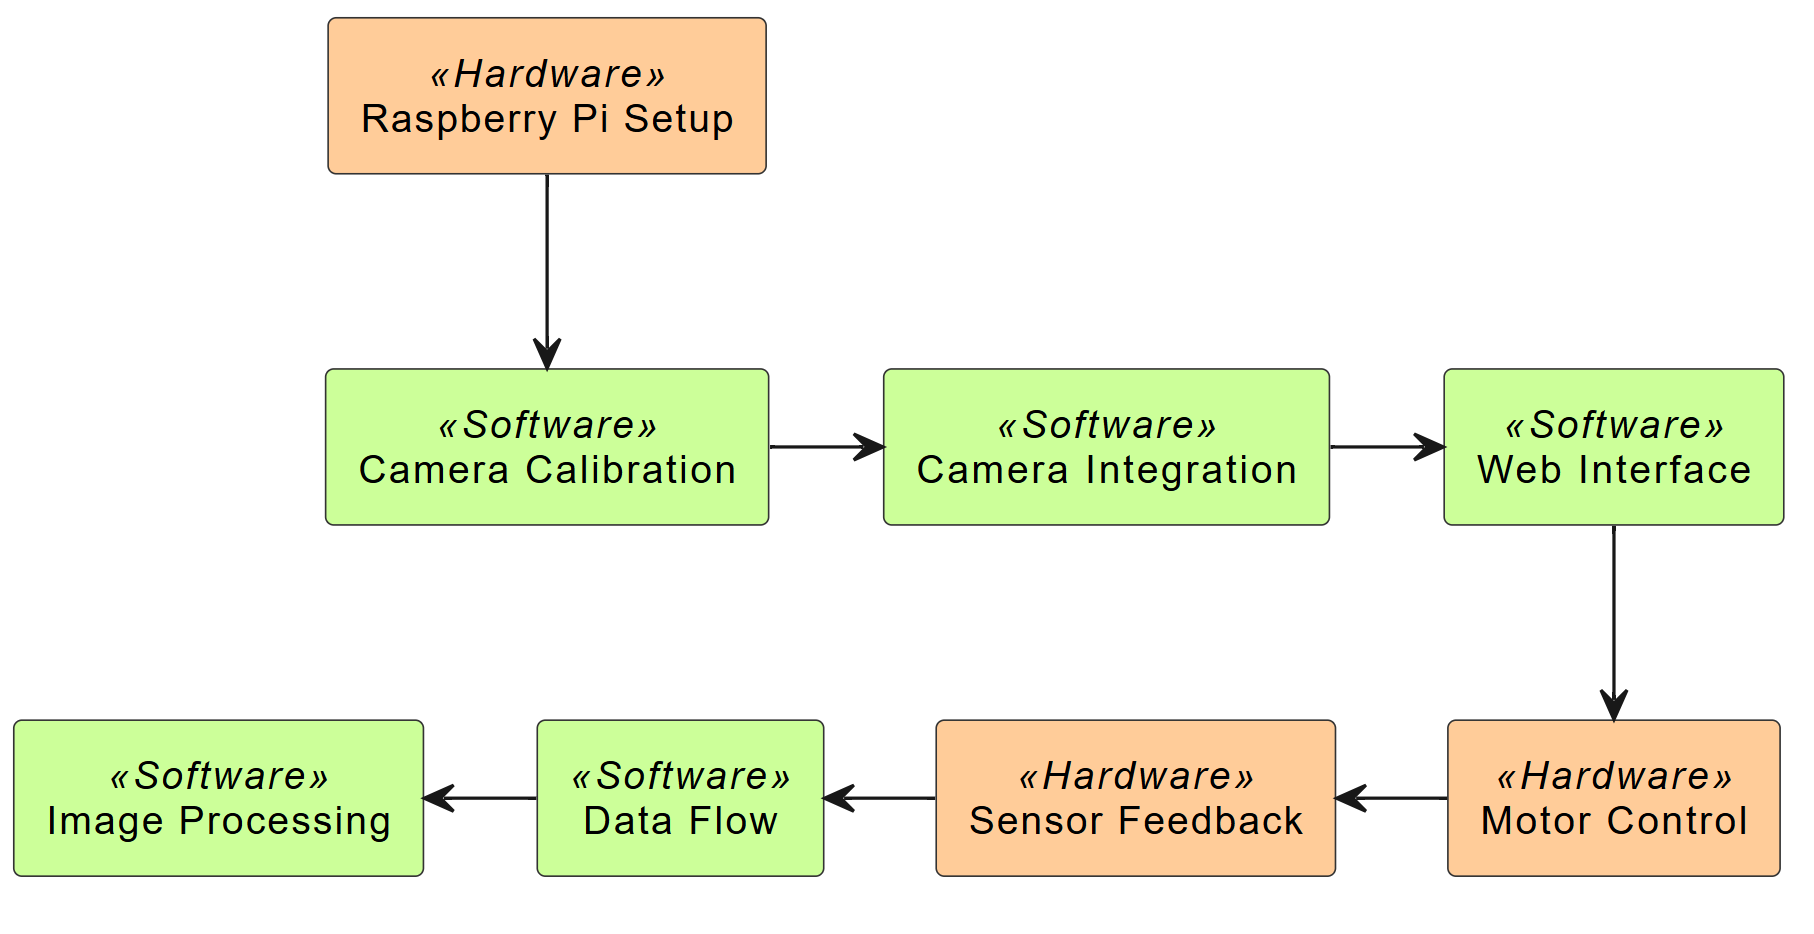
\includegraphics[width=0.5\textwidth]{ch4/figs/hi.png}
	\caption{Illustration of the project production process.}
	\label{fig:moto}
\end{figure}

\begin{table}[ht]
\centering
\caption{System Architecture Components}
\label{tab:system_architecture}
\begin{tabular}{|p{5cm}|p{10cm}|}
	\hline
	\textbf{Component}          & \textbf{Description}                                                                                                              \\ \hline
	Microcontroller/Processor   & Manages computer vision algorithms and interfaces with hardware. Responsible for overall system control and data processing.      \\ \hline
	Web Camera                  & Provides real-time video feed for remote monitoring and vision tasks. Captures high-quality images for processing.                \\ \hline
	Motor and Drive System      & Four-wheel drive system for robot mobility. Includes motors and a motor controller for precise movement control.                  \\ \hline
	Fiducial Markers            & Visual markers (e.g., ArUco or AprilTag) placed in the environment to assist with localization and navigation.                    \\ \hline
	Web-based Control Interface & Allows remote control of the robot’s movements and camera functions, with video streaming capabilities.                           \\ \hline
	Power Supply                & Provides electrical power to all components of the system. Needs to support extended operation and peak power demands.            \\ \hline
	Chassis                     & Physical structure of the robot that houses and protects all components. Designed for durability and optimal component placement. \\ \hline
	Sensors                     & Additional sensors for environmental awareness (e.g., ultrasonic sensors, IMU, GPS).                                              \\ \hline
	Communication Module        & Enables wireless communication between the robot and the control interface, supporting long-range and reliable data transmission. \\ \hline
\end{tabular}
\end{table}
